% Methodology
\section{Unified Preprocessing and Validation Pipeline}
\label{sec:methodology}

Before any detector was initialized or trained, the frozen KITTI and Waymo data were
transformed into a single, reproducible object-detection pipeline. The work standardized
image geometry, bounding-box coordinates, class identities, annotation formats,
region-handling rules, augmentation behavior, framework configuration, and model-ready
data loading, so that every later model would receive semantically equivalent data under a
controlled experimental protocol. The complete preprocessing and validation sequence is
summarized in Figure~\ref{fig:pipeline}.

\begin{figure}[t]
    \centering
    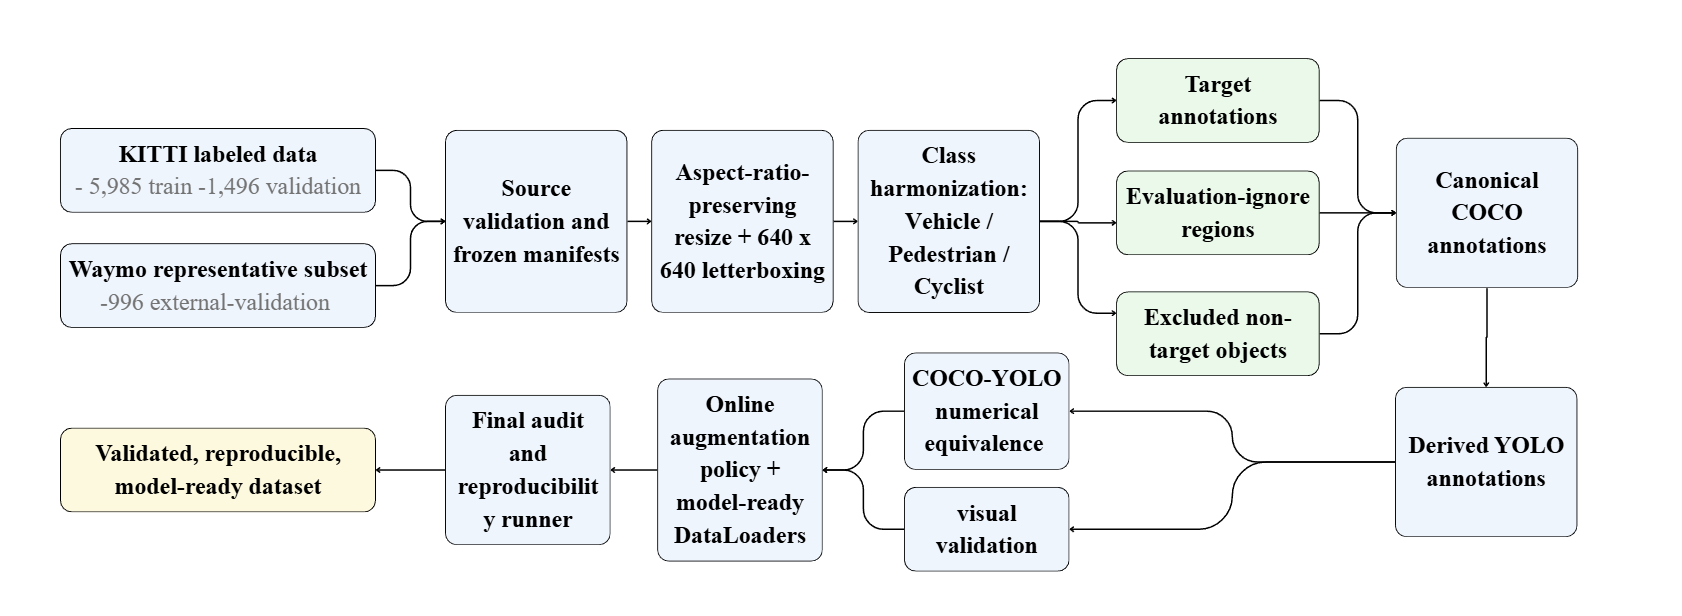
\includegraphics[width=\linewidth]{figures/pipeline.png}
    \caption{Unified preprocessing and validation pipeline. Frozen KITTI training and
    validation partitions and the Waymo external-validation subset are processed through
    common image standardization, class harmonization, annotation conversion, independent
    validation, controlled augmentation, model-ready loading, and a final reproducibility
    audit.}
    \label{fig:pipeline}
\end{figure}

\subsection{Experimental Roles and Leakage Prevention}
\label{sec:methodology_roles}

The experimental roles of the three partitions were fixed before model development. KITTI
train ($5{,}985$ images) is the only partition permitted to update model parameters. KITTI
validation ($1{,}496$ images) is reserved for in-domain validation, checkpoint comparison,
and model-development decisions. The representative Waymo subset ($996$ FRONT-camera
images from $25$ driving segments) is reserved exclusively for final cross-dataset
evaluation. Waymo data are not used for training, fine-tuning, early stopping,
hyperparameter optimization, threshold selection, checkpoint selection, or
augmentation-source sampling, preventing external-domain information from influencing the
learned parameters or the selection of the final model. The information-flow boundary is
illustrated in Figure~\ref{fig:partition_roles}.

\begin{figure}[t]
    \centering
    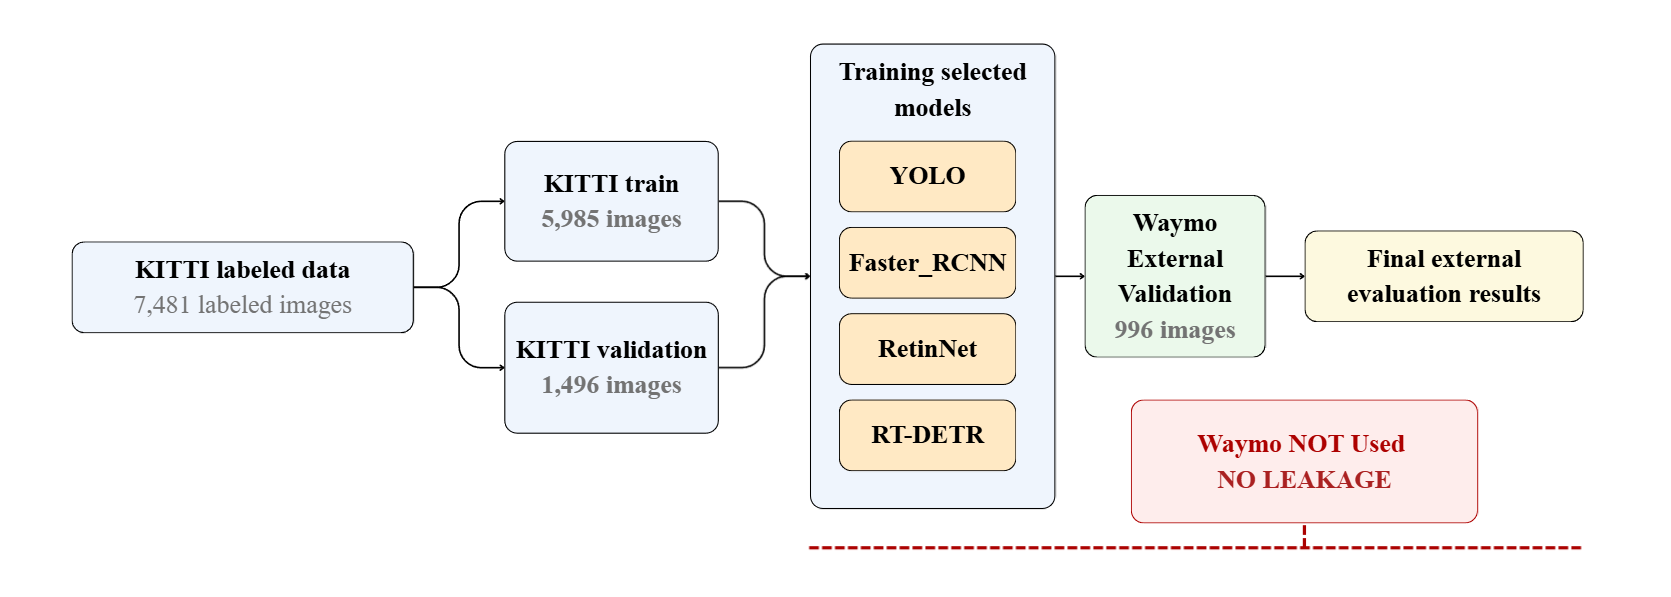
\includegraphics[width=\linewidth]{figures/partition_roles.png}
    \caption{Experimental partition roles and information-flow restrictions. KITTI train
    supports parameter learning, KITTI validation supports in-domain model development, and
    Waymo remains isolated until the final external evaluation of the selected model.}
    \label{fig:partition_roles}
\end{figure}

The Waymo subset preserves twelve images with no Vehicle, Pedestrian, or Cyclist
annotations; these target-negative scenes are retained intentionally because they support
later false-positive analysis under shifted driving conditions, and their empty labels are
treated as valid annotations rather than missing data.

\subsection{Image Standardization and Bounding-Box Transformation}
\label{sec:methodology_standardization}

The source datasets have substantially different image geometries: KITTI object-detection
images are typically wide road scenes close to $1{,}200\times370$ pixels, whereas the
selected Waymo FRONT-camera images have dimensions of $1{,}920\times1{,}280$ pixels.
Every source image was therefore converted to a common $640\times640$ representation using
aspect-ratio-preserving letterboxing. For an image of width $W$ and height $H$, the resize
factor was defined as $\min(640/W, 640/H)$; the resized image was centered within a
$640\times640$ canvas, and unused pixels were filled with the neutral gray value $114$ in
each channel. This procedure avoids geometric stretching while providing a fixed input
size for all detector families. The processed images were saved as PNG files to avoid
additional lossy compression.

Every bounding box was transformed using the exact scale and padding offsets applied to
its image, and transformed coordinates were checked against the processed-image boundary.
Across the complete set of $8{,}477$ images, preprocessing produced no missing outputs, no
invalid target boxes, no out-of-bound target boxes, and no clipped target boxes. Typical
KITTI images were resized to approximately $640\times193$ pixels with about $223$ pixels
of top padding and $224$ pixels of bottom padding, while Waymo images were resized to
approximately $640\times427$ pixels with about $106$ pixels of top and bottom padding.
Independent dry-run images confirmed that road content remained undistorted and that
transformed boxes remained attached to their source objects.

\subsection{Annotation Harmonization and Region Policy}
\label{sec:methodology_regions}

A common three-class taxonomy was frozen for the entire project. In the canonical COCO
representation these classes use identifiers $1$, $2$, and $3$, while in the derived YOLO
representation they use identifiers $0$, $1$, and $2$; the distinction preserves
compatibility with Torchvision, where class zero is reserved for background, and with
YOLO, where foreground classes begin at zero. The resulting combined target set contains
$49{,}678$ Vehicle boxes, $11{,}836$ Pedestrian boxes, and $2{,}391$ Cyclist boxes, for a
total of $63{,}905$ target annotations.

Target annotations were kept separate from two additional region types. KITTI DontCare
annotations were preserved as evaluation-ignore regions because eligible detections inside
these areas may be suppressed during evaluation instead of being counted as false
positives. KITTI Tram and Misc annotations were preserved as excluded non-target audit
regions; they are not project targets and do not automatically suppress false positives.
Waymo Sign and Unknown are assigned to the excluded category if encountered. The finalized
sidecars contain $11{,}295$ evaluation-ignore regions and $1{,}484$ excluded non-target
regions, none of which is inserted into the canonical COCO or derived YOLO target labels,
ensuring that training targets, evaluation suppression rules, and audit-only regions cannot
be confused by later model code.

\subsection{Canonical COCO and Derived YOLO Representations}
\label{sec:methodology_representations}

COCO was selected as the canonical target representation because it provides explicit image
and annotation identifiers, absolute pixel coordinates, named categories, and broad
framework compatibility. Three partition-specific files were created
(\texttt{kitti\_train.json}, \texttt{kitti\_val.json}, and
\texttt{waymo\_external.json}) with bounding boxes in the standard $[x, y, w, h]$
representation in absolute coordinates on the processed $640\times640$ images. The
canonical files contain $5{,}985$ KITTI training images with $31{,}294$ annotations,
$1{,}496$ KITTI validation images with $7{,}792$ annotations, and $996$ Waymo external
images with $24{,}819$ annotations (all $996$ Waymo records retained, including the twelve
with zero target annotations).

YOLO labels were derived from the canonical COCO files rather than generated independently
from the original sources. Each row stores the class identifier followed by normalized
center-$x$, center-$y$, width, and height values, serialized with ten decimal places, with
one label file per processed image (so the twelve target-negative Waymo images have valid
empty label files rather than absent labels). A framework adapter mirrors the validated
YOLO files beneath sibling images and labels directories expected by Ultralytics-style
pipelines; the adapter files are byte-identical to the canonical YOLO labels and do not
introduce a second ground-truth source.

\subsection{Numerical and Visual Validation}
\label{sec:methodology_validation}

A complete numerical equivalence test compared all $63{,}905$ canonical COCO boxes with
their serialized YOLO counterparts. Each YOLO box was reconstructed in processed-image
pixel coordinates and matched to the corresponding COCO box by image and class using
minimum-cost bipartite matching, so the result did not depend on annotation order. All
$63{,}905$ boxes were matched and classified as equivalent, with zero mismatched images;
the maximum normalized coordinate error was approximately $5.0\times10^{-11}$, the maximum
reconstructed pixel error approximately $4.8\times10^{-8}$ pixels, and the minimum
reconstructed intersection-over-union $0.9999998$. Visual comparisons for crowded,
cyclist-rich, pedestrian-rich, mixed, and target-negative scenes coincided between COCO
and YOLO overlays, with no boxes entering the gray letterbox padding.

\subsection{Augmentation Policy and Model-Ready Data Loading}
\label{sec:methodology_augmentation}

A conservative online augmentation policy was frozen for training. Augmentation is enabled
only for KITTI train and is disabled for KITTI validation and Waymo external evaluation;
no permanent augmented dataset is created. The permitted transformations are horizontal
flipping (probability $0.50$), brightness and contrast adjustment ($0.50$), HSV adjustment
($0.30$), and mild Gaussian blur ($0.10$). Vertical flipping, random cropping, arbitrary
rotation, perspective transformation, random scaling, shear, Mosaic, MixUp, Copy-Paste,
and Cutout are disabled, reducing unrealistic road geometry and preventing one detector
family from receiving framework-specific augmentation advantages. The random state is
derived from the base seed $42$, the training epoch, and the global image identifier,
making each augmented view reproducible.

A framework-neutral PyTorch dataset loader was implemented from the canonical COCO files,
returning a three-channel $640\times640$ float tensor, absolute XYXY boxes, canonical
labels, image and source identifiers, box areas, crowd flags, evaluation-ignore boxes,
excluded-object boxes, partition metadata, and an augmentation trace when training
augmentation is enabled, together with a detection-specific collation function supporting
variable numbers of objects per image. Smoke tests confirmed the expected partition
lengths, valid tensor and box shapes, finite values, correct class IDs, deterministic
validation behavior, valid target-negative handling, and a guard that prevents augmentation
from being enabled on validation or external partitions.

\subsection{Final Dataset Composition and Audit}
\label{sec:methodology_audit}

The final prepared dataset contains $8{,}477$ processed images and $63{,}905$ target
annotations, occupying approximately $2.1$~GiB. A read-only final audit combined the
outputs of all earlier validation stages with direct checks of physical images, COCO files,
canonical YOLO labels, framework labels, sidecar regions, manifests, issue files, and
visual artifacts, confirming exact class totals, valid empty labels for the twelve negative
images, zero partition overlap, complete COCO--YOLO equivalence, and correct DataLoader
behavior. The audit concluded with zero unresolved issues and a final status of PASSED.
